% !TEX root =../main.tex


\chapter{Beispiel}

Hier etwas Text zur Einleitung. Ye ist meine absolute Lieblings Ye.


\section{Ziel der Arbeit}

Ja, wir finden auch, dass man über die Copy noch mal reden sollte. Das hier kann es jedenfalls nicht sein. Das klingt ja wie auf dem Totenbett getextet. Da muss wesentlich mehr Produktaussage rein. Ja, wir finden auch, dass man über die Copy noch mal reden sollte. Das hier kann es jedenfalls nicht sein. Das klingt ja wie auf dem Totenbett getextet. Da muss wesentlich mehr Produktaussage rein. Ja, wir finden auch, dass man über die Copy noch mal reden sollte.


\subsection{Motivation}

Ja, wir finden auch, dass man über die Copy noch mal reden sollte. Das hier kann es jedenfalls nicht sein. Das klingt ja wie auf dem Totenbett getextet. Da muss wesentlich mehr Produktaussage rein. Ja, wir finden auch, dass man über die Copy noch mal reden sollte. Das hier kann es jedenfalls nicht sein. Das klingt ja wie auf dem Totenbett getextet. Da muss wesentlich mehr Produktaussage rein. Ja, wir finden auch, dass man über die Copy noch mal reden sollte.


\subsubsection{Meine Motivation}

Ja, wir finden auch, dass man über die Copy noch mal reden sollte. Das hier kann es jedenfalls nicht sein. Das klingt ja wie auf dem Totenbett getextet. Da muss wesentlich mehr Produktaussage rein. Ja, wir finden auch, dass man über die Copy noch mal reden sollte. Das hier kann es jedenfalls nicht sein. Das klingt ja wie auf dem Totenbett getextet. Da muss wesentlich mehr Produktaussage rein. Ja, wir finden auch, dass man über die Copy noch mal reden sollte.


\paragraph{Ein Paragraph}

Ja, wir finden auch, dass man über die Copy noch mal reden sollte. Das hier kann es jedenfalls nicht sein. Das klingt ja wie auf dem Totenbett getextet. Da muss wesentlich mehr Produktaussage rein. Ja, wir finden auch, dass man über die Copy noch mal reden sollte. Das hier kann es jedenfalls nicht sein. Das klingt ja wie auf dem Totenbett getextet. Da muss wesentlich mehr Produktaussage rein. Ja, wir finden auch, dass man über die Copy noch mal reden sollte.


\subparagraph{Ein Unterparagraph}

Ja, wir finden auch, dass man über die Copy noch mal reden sollte. Das hier kann es jedenfalls nicht sein. Das klingt ja wie auf dem Totenbett getextet. Da muss wesentlich mehr Produktaussage rein. Ja, wir finden auch, dass man über die Copy noch mal reden sollte. Das hier kann es jedenfalls nicht sein. Das klingt ja wie auf dem Totenbett getextet. Da muss wesentlich mehr Produktaussage rein. Ja, wir finden auch, dass man über die Copy noch mal reden sollte.


\section{Textauszeichnung (logisches Markup)}

Es können beliebig viele Befehle definiert werden, um Text besonders hervorzuheben. Zwei vordefinierte Befehle stehen bereits zur Verfügung. Ein Befehl für generelles hervorheben von Text und ein Befehl, um Quellcode-Begriffe hervorzuheben. Falls weitere Typen der Textauszeichnung gewünscht sind, können diese einfach hinzugefügt werden.

\emph{Hervorgehobener Text}

\code{Begriffe aus dem Quellcode}


\section{Aufzählungen}

Aufzählung mit Stichpunkten:

\begin{itemize}
	\item Erster Punkt
	\item Zweiter Punkt
	\item Dritter Punkt
\end{itemize}

Nummerierte Aufzählung.

\begin{enumerate}
	\item Erster Punkt
	\item Zweiter Punkt
	\item Dritter Punkt
\end{enumerate}


\section{Abbildungen}

In der Abbildung \vref{fig:wursthund} ist der so genannte Wursthund in seiner natürlichen Umgebung zu sehen.

\begin{figure}[htbp]
	\centering
	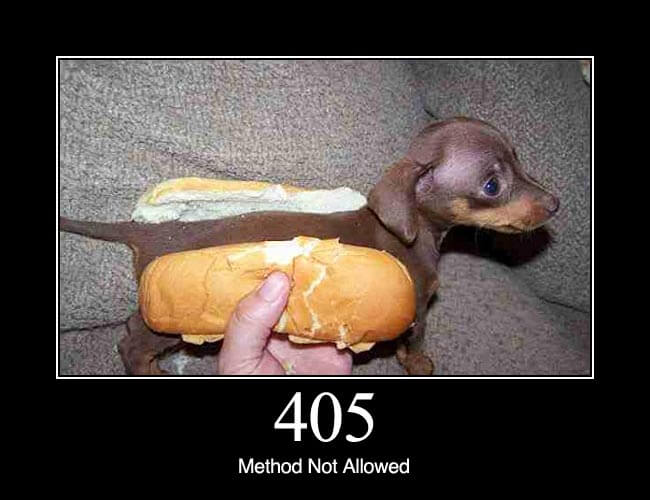
\includegraphics[width=0.7\textwidth]{bilder/wursthund.jpg}
	\caption{Wursthund}
	\label{fig:wursthund}
\end{figure}


\section{Tabellen}

In diesem Abschnitt wird das Erstellen von Tabellen in \latex erläutert. Bevor das Erstellen der eigentlichen Tabellen erläutert wird, wird ein Hinweis zur Konfiguration des Texteditors TeXworks gegeben. Dieser ist optional und ist für die Nutzung dieser Vorlage nicht notwendig.

Anschließend wird anhand von Beispielen aufgezeigt, wie Tabellen mit variabler und fester Spaltenbreite erzeugt werden. Darüber hinaus wird dargestellt wie lange Tabellen, die sich über mehrere Seiten erstrecken, erstellt werden können.


\subsection{Konfiguration TeXworks}

Um Tabellen im Quellcode lesbar formatieren zu können, ist es zu empfehlen eine Editor-Schriftart mit fester breite zu verwenden.

Hierfür muss lediglich in TeXworks unter \code{Bearbeiten} $\rightarrow$ \code{Einstellungen} der Einstellungsdialog geöffnet werden. Hier kann in dem Reiter \code{Editor}, eine Schriftart ausgewählt werden. Schriftarten mit fester breite enthalten meistens das Wort \emph{Mono} im Namen. Eine geeignete Schriftart zur Verwendung in TeXworks ist \code{Ubuntu Mono}. Abbildung \vref{fig:einstellungen-schriftart} zeigt den Einstellungsdialog zur Auswahl der Schriftarten.

\begin{figure}
	\centering
	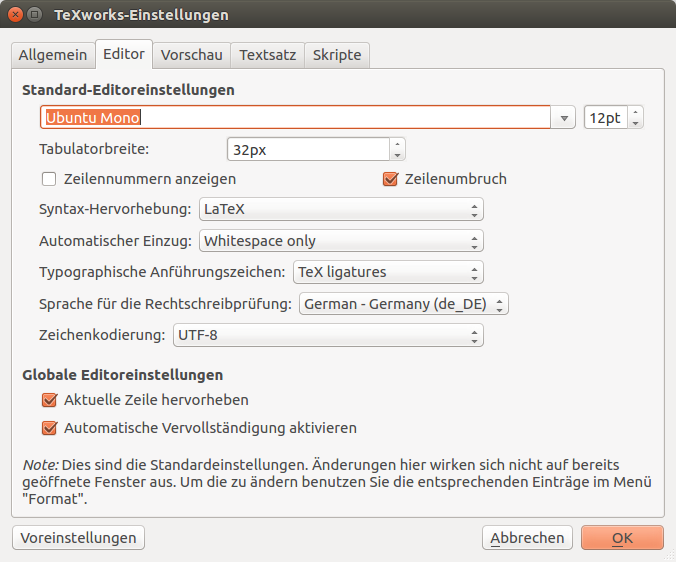
\includegraphics[width=0.7\textwidth]{bilder/einstellungen-schriftart.png}
	\caption{Einstellungsdialog für Schriftart in TeXworks}
	\label{fig:einstellungen-schriftart}
\end{figure}


\subsection{Tabellen mit variabler Spaltenbreite}

Ein Beispiel für eine Tabelle, mit variabler Spaltenbreite, ist durch Tabelle \vref{tab:variable-breite} dargestellt.

\begin{table}[htbp]
\centering
\begin{tabular}{l l l}
\toprule
Ziel            & Abfahrt      & Dauer \\
\midrule
Frankfurt       & stündlich    & 3:20 \\
Berlin          & stündlich    & 5:40 \\
Hamburg         & alle 5\,h    & 5:20 \\
\bottomrule
\end{tabular}
\caption{Tabelle mit variabler Spaltenbreite}
\label{tab:variable-breite}
\end{table}


\subsection{Tabellen mit fester Spaltenbreite}

Ein Beispiel für eine Tabelle, mit fester Spaltenbreite, ist durch Tabelle \vref{tab:feste-breite} dargestellt.

\begin{table}[htbp]
\centering
\begin{tabular}{p{3.5cm} p{5.5cm}}
\toprule
\textbf{Spalte 1}  & \textbf{Spalte 2}\\
\midrule
\textbf{Eintrag 1} & \textbf{Eintrag 2}\\
Daten              & Daten\\
Daten              & Daten\\
Daten              & Daten\\
\midrule
\textbf{Eintrag 1} & \textbf{Eintrag 2}\\
Daten              & Daten\\
Daten              & Daten\\
Daten              & Daten\\
\bottomrule
\end{tabular}
\caption{Tabelle mit fester Spaltenbreite}
\label{tab:feste-breite}
\end{table}


\subsection{Tabellen über mehrere Seiten}

Eine lange Tabelle, welche sich über mehrere Seiten erstrecken kann ist in Tabelle \ref{tab:lange-tabelle} dargestellt.

\begin{longtable}{p{2cm} p{2cm} p{2cm} p{2cm} p{2cm}}
\toprule
\textbf{\O min}& \textbf{\O max}& \textbf{Wert 1}& \textbf{Wert 2}& \textbf{Wert 3}\\
\midrule
 6& 10&  56& 100& 20,00\\
 6& 10& 100& 150& 20,00\\
 6& 10& 150& 200& 20,00\\
 6& 10& 200& 250& 20,00\\
 6& 10& 250& 300& 20,00\\
 6& 10& 300& 350& 20,00\\
 6& 10& 350& 400& 20,00\\
10& 14&  63& 100& 20,00\\
10& 14& 100& 150& 20,00\\
10& 14& 150& 200& 20,00\\
10& 14& 200& 250& 20,00\\
10& 14& 250& 300& 20,00\\
10& 14& 300& 350& 20,00\\
10& 14& 350& 400& 20,00\\
\bottomrule
\caption{Lange Tabelle}
\label{tab:lange-tabelle}
\end{longtable}


\section{Verweise}

Es existieren mehrere Arten auf Objekte zu verweisen.

Abbildungsnummer: \ref{fig:wursthund}

Abbildungsnummer und relative Seitenzahl: \vref{fig:wursthund}

Seitenzahl: \pageref{fig:wursthund}

Relative Seitenzahl: \vpageref{fig:wursthund}


\section{Beschreibungsumgebung}

\begin{description}
\item[Begriff Nummer 1] Ja, wir finden auch, dass man über die Copy noch mal reden sollte. Das hier kann es jedenfalls nicht sein. Das klingt ja wie auf dem Totenbett getextet. Da muss wesentlich mehr Produktaussage rein. Ja, wir finden auch, dass man über die Copy noch mal reden sollte. Das hier kann es jedenfalls nicht sein. Das klingt ja wie auf dem Totenbett getextet. Da muss wesentlich mehr Produktaussage rein. Ja, wir finden auch, dass man über die Copy noch mal reden sollte.
\item[Begriff Nummer 2] Ja, wir finden auch, dass man über die Copy noch mal reden sollte. Das hier kann es jedenfalls nicht sein. Das klingt ja wie auf dem Totenbett getextet. Da muss wesentlich mehr Produktaussage rein. Ja, wir finden auch, dass man über die Copy noch mal reden sollte. Das hier kann es jedenfalls nicht sein. Das klingt ja wie auf dem Totenbett getextet. Da muss wesentlich mehr Produktaussage rein. Ja, wir finden auch, dass man über die Copy noch mal reden sollte.
\end{description}


\section{Fußnoten}

Zu diesem Satz existiert eine Fußnote.\footnote{Großartig! Du hast sie gefunden.} Sieh nach, ob du sie finden kannst.


\section{Quellenangabe}

Dieser Abschnitt zeigt, wie in \latex auf literarische Quellen verwiesen werden kann. Indem diese Funktionalitäten genutzt werden, ist \latex des Weiteren in der Lage, automatisch ein Literaturverzeichnis zu erstellen.

Bevor die Befehle zum Verweisen auf Literaturquellen erläutert werden, wird die dafür nötige Konfiguration im Editor TeXworks dargestellt. Falls ein anderer Editor für die Bearbeitung dieser Vorlage zum Einsatz kommt, kann der Unterabschnitt zur Konfiguration übersprungen werden.


\subsection{Konfiguration in TeXworks}

Diese Vorlage nutzt \code{biber} als Backend für das Verwalten von Literaturquellen und das erstellen von Literaturverweisen. Leider ist \code{biber} in TeXworks nicht vorkonfiguriert, aber dies kann mit wenig Arbeit nachgeholt werden.

Um \code{biber} zu konfigurieren, öffnen Sie die Einstellungen unter \code{Bearbeiten} $\rightarrow$ \code{Einstellungen}. Hier klicken Sie auf den Reiter \code{Skripte}, so wie in Abbildung \vref{fig:konfiguration-biber-01} dargestellt.

\begin{figure}
	\centering
	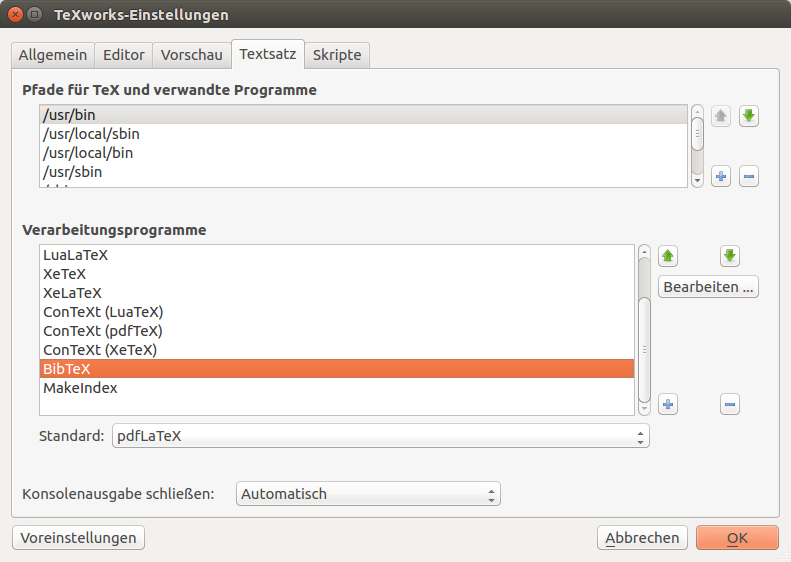
\includegraphics[width=0.7\textwidth]{bilder/konfiguration-biber-01.png}
	\caption{Konfiguration Literatur-Backend}
	\label{fig:konfiguration-biber-01}
\end{figure}

Klicken Sie auf \code{Bearbeiten} und tragen Sie, in dem sich öffnenden Fenster, in der Zeile \code{Befehl/Datei} den Wert \enquote{\code{biber}} ein. Ihre vorgenommenen Einstellungen, sollten denen in Abbildung \vref{fig:konfiguration-biber-02} entsprechen.

\begin{figure}
	\centering
	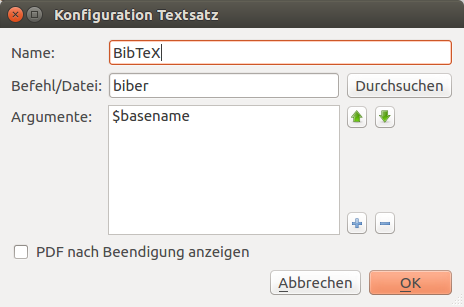
\includegraphics[width=0.7\textwidth]{bilder/konfiguration-biber-02.png}
	\caption{biber als Backend einsetzen}
	\label{fig:konfiguration-biber-02}
\end{figure}

Nun können über die grafische Oberfläche des Editors TeXworks literarische Quellen verwaltet und referenziert werden.

Es ist zu beachten, dass jedes mal wenn eine, noch nicht zuvor verwendete, literarische Quelle verwendet wird, folgende Anwendungen ausgeführt werden müssen: \code{pdfLaTeX} $\rightarrow$ \code{BibTeX} $\rightarrow$ \code{pdfLaTeX}. Dies ist ebenfalls in Abbildung \vref{fig:run-biber} zu sehen.

\begin{figure}
	\centering
	
\includegraphics[width=0.7\textwidth]{bilder/run-biber-01.png}
	
\includegraphics[width=0.7\textwidth]{bilder/run-biber-02.png}
	
\includegraphics[width=0.7\textwidth]{bilder/run-biber-01.png}
	\caption{Ausführung pdfLaTeX und BibTeX}
	\label{fig:run-biber}
\end{figure}


\subsection{Literaturverweise}

Ja, wir finden auch, dass man über die Copy noch mal reden sollte. Das hier kann es jedenfalls nicht sein. Das klingt ja wie auf dem Totenbett getextet. Da muss wesentlich mehr Produktaussage rein. Ja, wir finden auch, dass man über die Copy noch mal reden sollte. Das hier kann es jedenfalls nicht sein. Das klingt ja wie auf dem Totenbett getextet. Da muss wesentlich mehr Produktaussage rein. Ja, wir finden auch, dass man über die Copy noch mal reden sollte. \cite{angenendt}

\cite{angenendt,companion,vazques-de-parga,springer}
\footcite{angenendt}

\cite[5-12]{angenendt} % Quellverweis unformatiert

\parencite{angenendt} % Quellverweis in Klammern

\textcite{angenendt} % Quellverweis im Fließtext

Quelle als Fußnote.\footcite{angenendt} % Quellverweis als Fußnote


% Wörtliches Zitat

% Längeres wörtliches Zitat


\section{Quellcode}